\documentclass{article}

\usepackage[polish]{babel}
\usepackage{polski}
\usepackage[utf8]{inputenc}
\usepackage{longtable}
\usepackage{array}
\usepackage{enumitem}
\usepackage{makecell}
\usepackage{amsmath}
\usepackage{longtable}
\usepackage{graphicx}
\usepackage{float}
\usepackage{listings}
\usepackage[colorlinks=true, linkcolor=black]{hyperref}
\usepackage[letterpaper,top=2cm,bottom=2cm,left=3cm,right=3cm,marginparwidth=1.75cm]{geometry}

\renewcommand{\familydefault}{\sfdefault}

\setcounter{tocdepth}{2}

\title{Systemy ekspertowe: Nieruchomości \\ \large{Opis projektu}}
\author{Michalina Majewska
	\and Hubert Malinowski
	\and Igor Staręga
	\and Jan Szablanowski}

\begin{document}
\maketitle
% \tableofcontents
% \newpage

\section{Cel projektu}
Celem projektu jest stworzenie systemu ekspertowego, który będzie wspomagał użytkowników w wyborze nieruchomości do zakupu lub wynajmu. System będzie analizował dane o ofertach sprzedaży nieruchomości oraz preferencje użytkownika. Następnie na ich podstawie będzie wnioskował, która oferta jest dla użytkownika najlepsza. System będzie również umożliwiał wnioskowanie przybliżone, co pozwoli na wybór najlepszej oferty nawet w przypadku braku pełnych danych.

Wynikiem projektu będzie aplikacja okienkowa, która pozwoli użytkownikom na wprowadzanie danych o preferencjach dotyczących nieruchomości oraz przeglądanie rekomendacji. Użytkownik będzie wprowadzał dane w formie dialogu z systemem, a system będzie prezentował oferty spełniające kryteria i informacje o wywnioskowanych preferencjach.

\section{Baza wiedzy systemu ekspertowego}

% TODO: Michalina i Jan

System ekspertowy będzie korzystał z bazy danych, przechowującej dane o nieruchomościach, pośrednikach nieruchomości, ofertach sprzedaży i wynajmu. Baza zostanie stworzona we współpracy z zespołem ekspertów dziedzinowych. Na podstawie danych z bazy i reguł system będzie w stanie generować rekomendacje dla użytkowników, odpowiadając na ich zapytania. W kolejnych sekcjach przedstawiono specyfikację rekordów, które będą przechowywane w bazie danych systemu ekspertowego.

\subsection{Specyfikacja rekordów}

\begin{table}[H]
    \caption{Format rekordów o typie \textit{nieruchomość}}
    \centering
    \begin{tabular}{|l|l|l|}
    \hline
    \textbf{Atrybut} & \textbf{Typ} & \textbf{Opis} \\
    \hline
    id & String & Unikalny identyfikator nieruchomości \\
    property\_type & String & Typ nieruchomości (mieszkanie, dom, działka, lokal użytkowy, biuro) \\
    street\_address & String & Nazwa ulicy i numer \\
    city & String & Nazwa miasta \\
    state & String & Region administracyjny \\
    postal\_code & String & Kod pocztowy \\
    country & String & Nazwa kraju \\
    latitude & Float & Współrzędna geograficzna szerokości \\
    longitude & Float & Współrzędna geograficzna długości \\
    total\_area & Float & Całkowita powierzchnia w metrach kwadratowych \\
    rooms & Integer & Liczba pokojów  \\
    bathrooms & Integer & Liczba łazienek \\
    year\_built & Integer & Rok budowy nieruchomości \\
    construction\_type & String & Rodzaj materiału konstrukcyjnego \\
    floors & Integer & Liczba pięter w budynku \\
    floor\_number & Integer & Numer piętra dla mieszkań \\
    has\_elevator & Boolean & Czy budynek posiada windę \\
    has\_parking & Boolean & Czy dostępny jest parking \\
    parking\_type & String & Rodzaj parkingu (garaż podziemny, ulica) \\ 
    pet\_policy & String & Opis polityki dotyczącej zwierząt \\
    furnished & Boolean & Czy nieruchomość jest umeblowana \\
    heating\_type & String & Rodzaj systemu ogrzewania \\
    energy\_rating & String & Ocena efektywności energetycznej \\
    flood\_risk & String & Ocena ryzyka powodziowego \\
    property\_condition & String & Ogólna ocena stanu nieruchomości \\
    description & String & Szczegółowy opis nieruchomości \\
    available\_from & DateTime & Data, od której nieruchomość jest dostępna \\
    last\_renovation\_date & DateTime & Data ostatniego remontu \\
    created\_at & TimeStamp & Czasu utworzenia rekordu \\
    updated\_at & TimeStamp & Czasu aktualizacji rekordu \\
    \hline
    \end{tabular}
    \label{tab:property_details}
\end{table}

\begin{table}[H]
    \caption{Format rekordów o typie \textit{pośrednik nieruchomości}}
    \centering
    \begin{tabular}{|l|l|l|}
    \hline
    \textbf{Atrybut} & \textbf{Typ} & \textbf{Opis} \\
    \hline
    id & String & Unikalny identyfikator pośrednika nieruchomości \\
    location & String & Lokalizacja (miasto) biura pośrednictwa \\
    full\_name & String & Imię i nazwisko pośrednika \\
    email & String & Adres e-mail pośrednika \\
    phone & String & Numer telefonu pośrednika \\
    license\_number & String & Numer licencji pośrednictwa \\
    specialization & String & Specjalizacja pośrednika (mieszkania, domy, działki, lokale, biura) \\ 
    \hline
    \end{tabular}
    \label{tab:agent_details}
\end{table}

\begin{table}[H]
    \caption{Format rekordów o typie \textit{oferta sprzedaży}}
    \centering
    \begin{tabular}{|l|l|l|}
    \hline
    \textbf{Atrybut} & \textbf{Typ} & \textbf{Opis} \\
    \hline
    id & String & Unikalny identyfikator oferty sprzedaży \\
    property\_id & String & Unikalny identyfikator sprzedawanej nieruchomości \\
    agent\_id & String & Unikalny identyfikator pośrednika sprzedaży \\
    status & String & Status oferty (aktywna, zakończona, wycofana) \\
    price & Float & Cena oferty \\
    negotiable & Boolean & Czy cena jest do negocjacji \\    
    max\_price & Float & Maksymalna cena do negocjacji \\
    min\_price & Float & Minimalna cena do negocjacji \\
    listing\_date & DateTime & Data wystawienia oferty \\
    expiration\_date & DateTime & Data wygaśnięcia oferty \\
    preffered\_payment\_method & String & Preferowana metoda płatności (gotówka, kredyt hipoteczny) \\
    \hline
    \end{tabular}
    \label{tab:sell_offer_details}
\end{table}

\begin{table}[H]
    \caption{Format rekordów o typie \textit{oferta wynajmu}}
    \centering
    \begin{tabular}{|l|l|l|}
    \hline
    \textbf{Atrybut} & \textbf{Typ} & \textbf{Opis} \\
    \hline
    id & String & Unikalny identyfikator oferty sprzedaży \\
    property\_id & String & Unikalny identyfikator sprzedawanej nieruchomości \\
    agent\_id & String & Unikalny identyfikator pośrednika sprzedaży \\
    status & String & Status oferty (aktywna, zakończona, wycofana) \\
    price & Float & Cena oferty \\
    negotiable & Boolean & Czy cena jest do negocjacji \\    
    max\_price & Float & Maksymalna cena do negocjacji \\
    min\_price & Float & Minimalna cena do negocjacji \\
    listing\_date & DateTime & Data wystawienia oferty \\
    expiration\_date & DateTime & Data wygaśnięcia oferty \\
    preffered\_payment\_method & String & Preferowana metoda płatności (gotówka, kredyt hipoteczny) \\
    \hline
    \end{tabular}
    \label{tab:sell_offer_details}
\end{table}

\section{Fakty}

\section{Definicje}

\section{Relacje między rekordami}


\section{Wnioskowanie}
Wnioskowanie będzie odbywać się w oparciu o odpowiedzi użytkownika na pytania systemu o preferencje dotyczące nieruchomości. Na podstawie tych odpowiedzi system będzie wnioskował, które oferty są dla użytkownika najlepsze. W poniższych przykładach przedstawiono dialog systemu z użytkownikiem oraz wnioski wyciągnięte na podstawie odpowiedzi. W docelowym rozwiązaniu wyjściem systemu będzie lista nieruchomości, które najlepiej spełniają preferencje użytkownika.
\\ \\
\noindent \textbf{Ekspertyza: Dobór odpowiedniej nieruchomości}\\
\noindent Czy szukasz nieruchomości na sprzedaż, która będzie odpowiednia dla Ciebie? (T/N) \textbf{T} \\
\noindent Czy preferujesz mieszkanie, które będzie gotowe do zamieszkania? (T/N) \textbf{T} \\
\noindent Czy interesuje Cię nieruchomość z rynku pierwotnego, czyli nową? (T/N) \textbf{N} \\
\noindent Czy zależy Ci na lokalizacji w centrum miasta, w pobliżu sklepów i restauracji? (T/N) \textbf{T} \\
\noindent Czy wykluczasz zakup nieruchomości w kamienicy z powodu jej wieku lub stanu? (T/N) \textbf{N} \\
MOIM ZDANIEM: Powinieneś rozważyć zakup mieszkania w nowoczesnym apartamentowcu w centrum, gdzie będziesz miał blisko do najważniejszych punktów miasta.\\
\textbf{EKSPERTYZA ZAKOŃCZONA}\\

\noindent \textbf{Ekspertyza: Wybór rodzaju najmu}\\
\noindent Czy rozważasz wynajęcie nieruchomości na krótki okres? (T/N) \textbf{T} \\
\noindent Czy preferujesz wynajem krótkoterminowy, np. przez platformy takie jak Airbnb? (T/N) \textbf{T} \\
\noindent Czy planujesz pobyt w wynajmowanej nieruchomości krótszy niż miesiąc? (T/N) \textbf{T} \\
MOIM ZDANIEM: Powinieneś rozważyć wynajem krótkoterminowy, np. przez popularne platformy rezerwacyjne typu AirBNB.\\
\textbf{EKSPERTYZA ZAKOŃCZONA}\\

\noindent \textbf{Ekspertyza: Ocena inwestycji w nieruchomość}\\
\noindent Czy rozważasz zakup nieruchomości pod inwestycję, z zamiarem jej późniejszego wynajmu? (T/N) \textbf{T} \\
\noindent Czy planujesz wynajmować nieruchomość na długoterminowy okres? (T/N) \textbf{T} \\
\noindent Czy preferujesz mieszkanie w dużym mieście, które może przyciągać wielu najemców? (T/N) \textbf{T} \\
\noindent Czy Twój budżet na zakup nieruchomości przekracza 500 tys. zł? (T/N) \textbf{N} \\
MOIM ZDANIEM: Powinieneś rozważyć zakup mniejszego mieszkania w rozwijającej się dzielnicy, która posiada dobrą komunikację i ma potencjał na przyszły wzrost wartości.\\
\textbf{EKSPERTYZA ZAKOŃCZONA}\\

\noindent \textbf{Ekspertyza: Wybór nieruchomości dla rodziny}\\
\noindent Czy poszukujesz nieruchomości, która będzie odpowiednia dla całej rodziny? (T/N) \textbf{T} \\
\noindent Czy masz dzieci, które będą korzystać z tej nieruchomości? (T/N) \textbf{T} \\
\noindent Czy interesuje Cię zakup domu jednorodzinnego, który zapewni przestronność? (T/N) \textbf{T} \\
\noindent Czy duży ogród jest dla Ciebie istotnym kryterium przy wyborze nieruchomości? (T/N) \textbf{T} \\
MOIM ZDANIEM: Powinieneś rozważyć zakup przestronnego domu z dużym ogrodem w spokojnej okolicy, idealnym dla rodziny.\\
\textbf{EKSPERTYZA ZAKOŃCZONA}\\

\noindent \textbf{Ekspertyza: Wybór nieruchomości do remontu}\\
\noindent Czy interesuje Cię zakup nieruchomości, którą będziesz mógł wyremontować według własnych potrzeb? (T/N) \textbf{T} \\
\noindent Czy masz doświadczenie w przeprowadzaniu remontów, czy wolisz zlecić to specjalistom? (T/N) \textbf{N} \\
\noindent Czy zależy Ci na niższej cenie zakupu nieruchomości, mimo potrzeby przeprowadzenia remontu? (T/N) \textbf{T} \\
MOIM ZDANIEM: Powinieneś rozważyć zakup nieruchomości, która jest w dobrym stanie, ale wymaga drobnych prac remontowych, co pozwoli Ci zaoszczędzić na zakupie.\\
\textbf{EKSPERTYZA ZAKOŃCZONA}\\

\noindent \textbf{Ekspertyza: Wybór lokalizacji nieruchomości}\\
\noindent Czy interesuje Cię zakup nieruchomości, która znajduje się w cichej i zielonej okolicy, z dala od miejskiego zgiełku? (T/N) \textbf{T} \\
\noindent Czy zależy Ci na bliskości szkół i przedszkoli, aby ułatwić codzienne życie? (T/N) \textbf{T} \\
\noindent Czy Twój budżet na zakup nieruchomości jest poniżej 500 tys. zł? (T/N) \textbf{T} \\
MOIM ZDANIEM: Powinieneś rozważyć zakup mieszkania na przedmieściach, które oferują spokój, bliskość parków i szkół, a także są tańsze niż w centrum miasta.\\
\textbf{EKSPERTYZA ZAKOŃCZONA}\\

\noindent \textbf{Ekspertyza: Zakup nieruchomości dla singla}\\
\noindent Czy poszukujesz nieruchomości na sprzedaż, która będzie odpowiednia dla Ciebie jako singla? (T/N) \textbf{T} \\
\noindent Czy preferujesz zakup mieszkania, które będzie dostosowane do Twoich indywidualnych potrzeb? (T/N) \textbf{T} \\
\noindent Czy zależy Ci na lokalizacji blisko pracy, aby oszczędzać czas na dojazdach? (T/N) \textbf{T} \\
\noindent Czy interesuje Cię małe mieszkanie, takie jak kawalerka lub studio? (T/N) \textbf{T} \\
MOIM ZDANIEM: Powinieneś rozważyć zakup kawalerki w pobliżu centrum miasta, co zapewni Ci wygodny dostęp do pracy i usług.\\
\textbf{EKSPERTYZA ZAKOŃCZONA}\\

\noindent \textbf{Ekspertyza: Wybór nieruchomości na wynajem krótkoterminowy}\\
\noindent Czy chcesz wynająć nieruchomość na krótki okres? (T/N) \textbf{T} \\
\noindent Czy zależy Ci na wynajmie krótkoterminowym, np. przez platformy turystyczne? (T/N) \textbf{T} \\
\noindent Czy nieruchomość ma znajdować się w popularnej turystycznie lokalizacji? (T/N) \textbf{T} \\
\noindent Czy masz wystarczający budżet, aby pokryć wyższe koszty utrzymania nieruchomości? (T/N) \textbf{T} \\
MOIM ZDANIEM: Powinieneś rozważyć zakup nieruchomości w popularnej turystycznie dzielnicy, która będzie miała duży potencjał wynajmu krótkoterminowego.\\
\textbf{EKSPERTYZA ZAKOŃCZONA}\\

\noindent \textbf{Ekspertyza: Sprzedaż mieszkania}\\
\noindent Czy planujesz sprzedaż nieruchomości, którą posiadasz? (T/N) \textbf{T} \\
\noindent Czy nieruchomość jest gotowa do sprzedaży, nie wymaga dodatkowych napraw lub remontów? (T/N) \textbf{T} \\
\noindent Czy zależy Ci na szybkiej sprzedaży, z uwagi na pilną potrzebę? (T/N) \textbf{T} \\
\noindent Czy masz odpowiednią cenę wyjściową, która może przyciągnąć kupców? (T/N) \textbf{N} \\
MOIM ZDANIEM: Powinieneś skonsultować cenę z rzeczoznawcą, aby ustalić konkurencyjną ofertę, która pomoże w szybszej sprzedaży.\\
\textbf{EKSPERTYZA ZAKOŃCZONA}\\

\noindent \textbf{Ekspertyza: Wynajem nieruchomości}\\
\noindent Czy chcesz wynająć nieruchomość, którą posiadasz? (T/N) \textbf{T} \\
\noindent Czy zamierzasz wynajmować nieruchomość innym osobom? (T/N) \textbf{T} \\
\noindent Czy interesuje Cię wynajem długoterminowy, np. na kilka lat? (T/N) \textbf{T} \\
\noindent Czy Twoja nieruchomość znajduje się w atrakcyjnej lokalizacji, która przyciągnie najemców? (T/N) \textbf{T} \\
MOIM ZDANIEM: Powinieneś rozważyć wynajem długoterminowy nieruchomości w dobrej lokalizacji, aby zapewnić stabilny dochód.\\
\textbf{EKSPERTYZA ZAKOŃCZONA}\\

\section{Interfejs użytkownika}
Interfejs graficzny systemu eksperckiego dotyczącego nieruchomości został wstępnie zaprojektowany przy użyciu bibliotek \texttt{Tkinter} oraz \texttt{CustomTkinter} w języku Python. Aplikacja działa na zasadzie konwersacji z użytkownikiem, w której system zadaje pytania typu Tak/Nie, a użytkownik odpowiada klikając odpowiedni przycisk.
\\ \\
Okno aplikacji składa się z dwóch głównych części:
\begin{itemize}
    \item \textbf{Panel czatu} -- scrollowalne pole, w którym pojawiają się dymki z pytaniami systemu oraz odpowiedziami użytkownika. Wiadomości systemowe są wyrównane do lewej i wyświetlane w jasnoszarych dymkach, natomiast odpowiedzi użytkownika są wyrównane do prawej i przedstawione w niebieskich dymkach.
    \item \textbf{Panel odpowiedzi} -- znajdujący się na dole interfejsu, zawiera dwa przyciski: \texttt{Tak} oraz \texttt{Nie}. Po kliknięciu jednego z nich odpowiedź użytkownika jest rejestrowana i wyświetlana w czacie, a system automatycznie przechodzi do kolejnego pytania.
\end{itemize}

\noindent Taki sposób komunikacji imituje naturalny dialog i zwiększa czytelność oraz przyjazność obsługi systemu dla użytkownika. Interfejs jest gotowy do rozbudowy o logikę wnioskowania oraz dodatkowe funkcjonalności.
\begin{figure}[H]
    \centering
    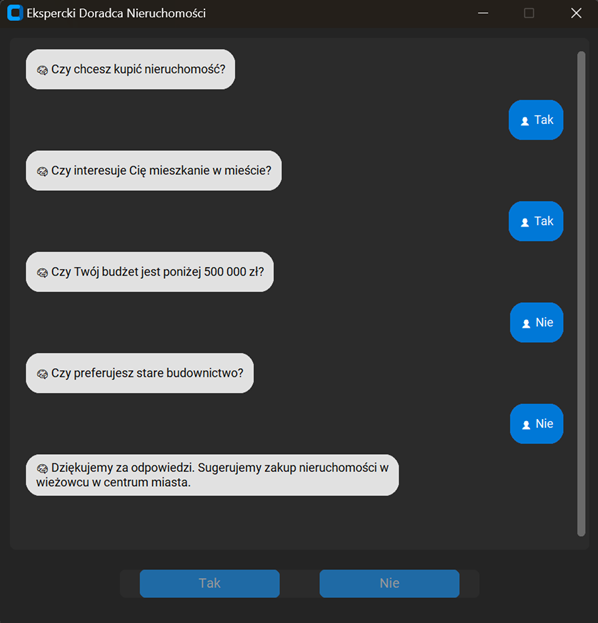
\includegraphics[width=.9\linewidth]{tex/fig/ui.png}
    \caption{Projekt interfejsu}
    
    \end{figure}

% TODO: Igor
\section{Wnioskowanie przybliżone}

%TODO: Hubert

\end{document}